%%%%%%%%%%%%%%%%%%%%%%% file template.tex %%%%%%%%%%%%%%%%%%%%%%%%%
%
% This is a template file for Web of Conferences Journal
%
% Copy it to a new file with a new name Surname_MESON2016.tex
% and use it as the basis for your article
%
%%%%%%%%%%%%%%%%%%%%%%%%%% EDP Science %%%%%%%%%%%%%%%%%%%%%%%%%%%%
%
%%%\documentclass[option comma separated list]{webofc}
%%%Three important options:
%%% "epj" for EPJ Web of Conferences Journal
%%% "twocolumn" for typesetting an article in two columns format (default one column)
\documentclass[epj]{webofc}
\usepackage[varg]{txfonts}   % Web of Conferences font
%
% Put here some packages required or/and some personnal commands
%
\woctitle{MESON2016 - the 14$^\textrm{th}$ International Workshop on Meson Production, Properties and Interaction}
%
%
\begin{document}
%
\selectlanguage{english}
\title{Insert your title here, in all titles capitalize only first letter. No trailing dot, please}

% insert email only for speaker/presenter
\author{First~Author\inst{1,3}\fnsep\thanks{\email{speaker@meson2016.pl}, give only for the presenter} \and
        Second~Author\inst{2} \and
        Third~Author\inst{3} 
% comment out the next line if not needed
       \\for the XXXXX Collaboration
}

\institute{Insert the first institution here (name, city, country)
\and
           the second here (try to fit each institution in one line)
\and
           Last institution
          }

\abstract{%Do not break line here!
  Insert your English abstract here. It should be as consise as possible, continuous text with no paragraph structure. Abstract should contain no references, formulae or figures.
}
%
\maketitle
%
\section{Introduction}
\label{intro}
Your text comes here. Please respect the following rules:
\begin{enumerate}
\item For larger collaborations, give only initials of the authors' first names, making sure to insert non breaking spaces where necessary, e.g. P.~A.~M.~Dirac. 
\item Remember that each comma in the text should be followed by a space.
\item Do not change spacings between article components, leave them default (we will rather accept a longer contribution than a re-formatted paper!).
\item When referring to particle species by their symbols, ALWAYS use math mode, also in the text, e.g. $K_0,\ \rho, B_s$.
\item All elements in all figures must be readable in print, thus too small axis labels or titles should be avoided. All figures should be of good quality (at least 300~dpi).
\item When referring to figures write ``in Fig.~\ref{fig-1}`` , when referring to tables write ``in Table~\ref{tab-1}``, when referring to other papers write ``in Ref.~\cite{RefJ}`` or simply ``in~\cite{RefJ}``, when referring to equations ``in Eq.~(3)`` and to sections ``in Sect.~\ref{sec-2}``.
\item Stick to the proposed format of bibliography items, add arXiv numbers ONLY for the papers that have not been published in journals. Use only approved abbreviations of journal titles.
\item Remember to embed all fonts into your final pdf file.
\end{enumerate}
\section{Section title}
\label{sec-1}
For bibliography use \cite{RefJ}
\subsection{Subsection title}
\label{sec-2}
Do not forget to give each section, subsection, subsubsection, and
paragraph a unique label (see Sect.~\ref{sec-1}).

For figures use syntax as below. of Fig.~\ref{fig-1}
\begin{figure}[ht]
% Use the relevant command for your figure-insertion program
% to insert the figure file.
\centering
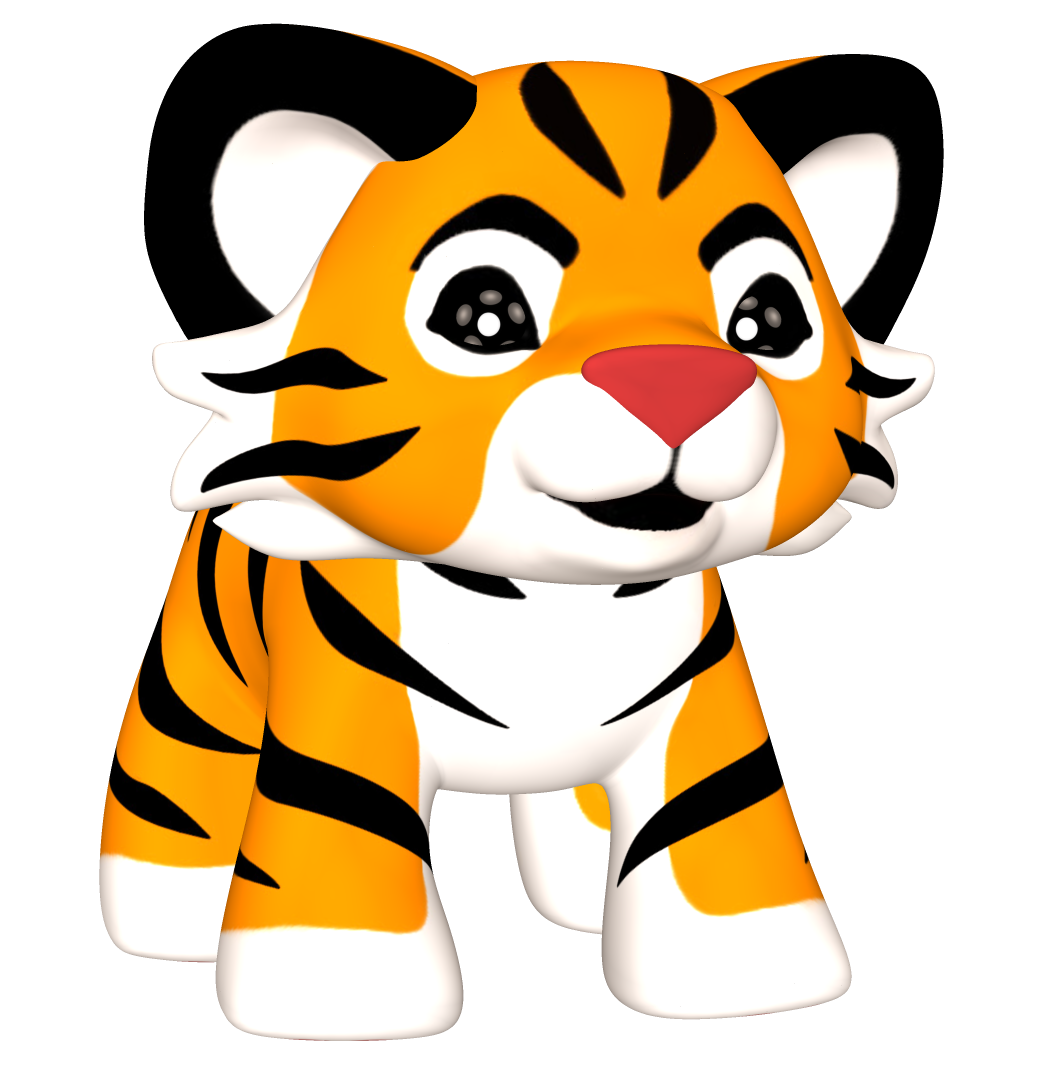
\includegraphics[width=4cm,clip]{MesonProcPackage/tiger}
\caption{Please write your figure caption here. Do not forget about the trailing dot.}
\label{fig-1}       % Give a unique label
\end{figure}

For figure with sidecaption legend use syntax of Fig.~\ref{fig-3}.
\begin{figure}[ht]
% Use the relevant command for your figure-insertion program
% to insert the figure file.
\centering
\sidecaption
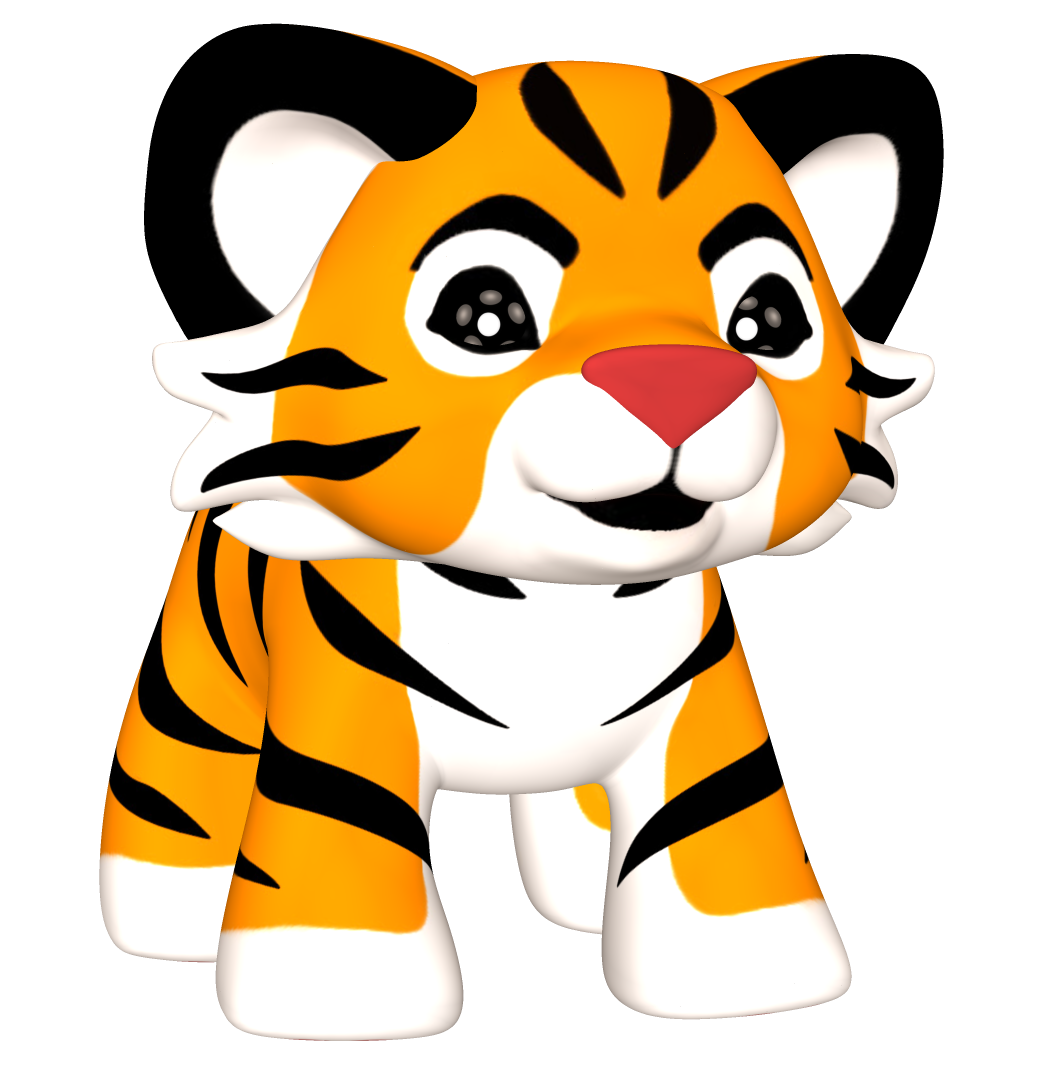
\includegraphics[width=5cm,clip]{MesonProcPackage/tiger}
\caption{Please write your figure caption here. Do not forget about the trailing dot.}
\label{fig-3}       % Give a unique label
\end{figure}

For tables use syntax in Table~\ref{tab-1}.
\begin{table}
\centering
\caption{Please write your table caption here.}
\label{tab-1}       % Give a unique label
% For LaTeX tables you can use
\begin{tabular}{lll}
\hline
first & second & third  \\\hline
number & number & number \\
number & number & number \\\hline
\end{tabular}
% Or use
\vspace*{5cm}  % with the correct table height
\end{table}

\begin{acknowledgement}
If you have nothing to write here, just remove the section.
\end{acknowledgement}
%
% BibTeX or Biber users please use (the style is already called in the class, ensure that the "woc.bst" style is in your local directory)
% \bibliography{name or your bibliography database}
%
% Non-BibTeX users please use
%
\begin{thebibliography}{00}
%
% and use \bibitem to create references.
%
\bibitem{RefJ}
% Format for Journal Reference
F.~Author~\textit{et al.}, Journal \textbf{Volume}, page numbers (year) {\em{no trailing dot!}}
% Format for books
\bibitem{RefB}
Book Author, \textit{Book title} (Publisher, place, year) page numbers {\em{no trailing dot!}}
% etc
\end{thebibliography}

\end{document}

% end of file template.tex

